\chapter{Umsetzung}
\label{chap:implementation}

Nachdem die Ziele der angestrebten TypeScript-Migration charakterisiert und die Anforderungen an den geplanten Transpiler ausgeführt wurden, soll im Folgenden der Entwurf und die Details der Implementierung ausgeführt werden. In Abschnitt~\ref{subsec:js-transpilers} wurden bereits die verbreitetsten Werkzeuge zur Transformation von JavaScript-Quelltexten ausführlich vorgestellt und verglichen. Auf Basis dieser Gegenüberstellung wurde schließlich Babel~\autocite{BABEL} als Grundlage der vorliegenden Umsetzung des Transpilers von Flow nach TypeScript gewählt.

\section{Software-Architektur}
\label{sec:software-architecture}
% \subsection{Konzeptioneller Aufbau des Transpilers}

Mit der Entscheidung den Übersetzer als Babel-Plugin zu implementieren, ist dessen Grundarchitektur bereits in Teilen festgelegt, da alle Plugins die vorgegebenen Programmschnittstellen von Babel erfüllen müssen. Bevor auf Einzelheiten der Umsetzung näher eingegangen wird, soll zunächst der grundsätzliche Aufbau der Anwendung skizziert werden. Abbildung~\ref{fig:architecture-overview} verschafft einen Überblick über die verschiedenen Komponenten des Systems und deren Beziehung zueinander.

\begin{figure}[tbp]
  \centering
  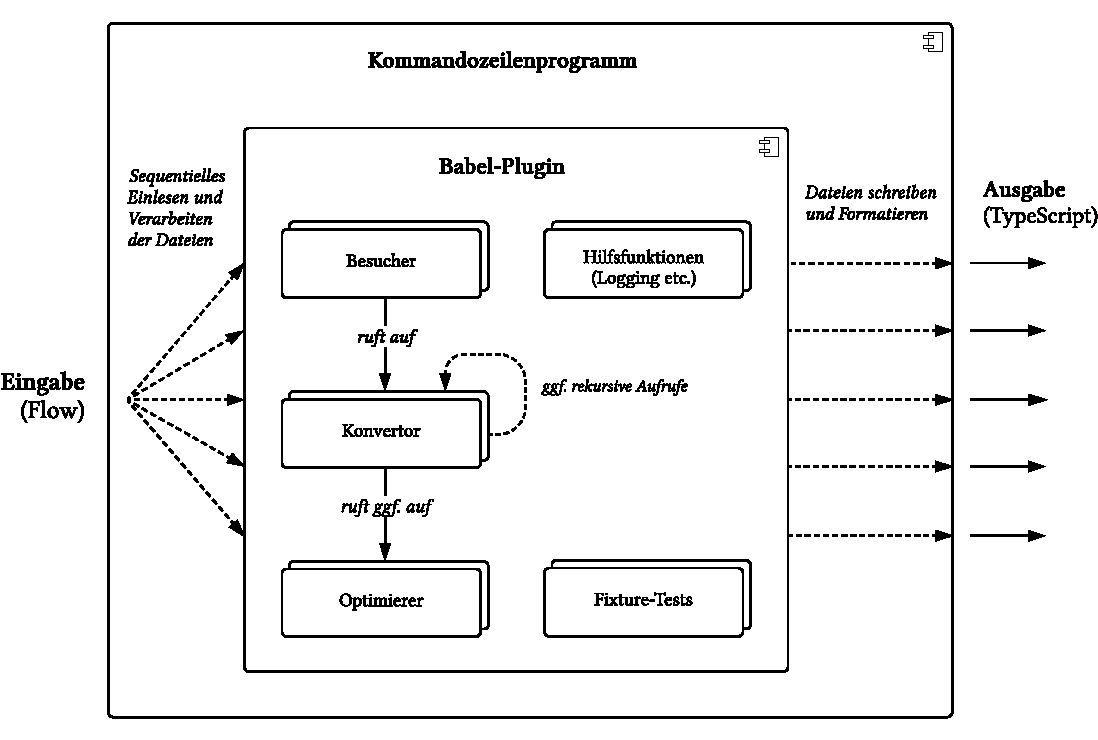
\includegraphics[width=0.92\textwidth]{src/4_Umsetzung/fig/architecture-overview.pdf}
	\caption{Überblick über die Komponenten des Transpilers}
	\label{fig:architecture-overview}
\end{figure}

Die Architektur gliedert sich in zwei Teile: Ein Kommandozeilenprogramm stellt die Benutzerschnittstelle dar, welche die Eingabe-Verzeichnisse bzw. -Dateien als Argument entgegen nimmt und verschiedene Optionen bereit stellt, um das Verhalten der Übersetzung zu beeinflussen. Die zweite Komponente ist ein Babel-Plugin, das die Transpilierung des Flow-Codes nach TypeScript realisiert. Das Kommandozeilenprogramm liest sukzessive alle Eingabeverzeichnisse bzw. -dateien ein und startet intern die Transpilierung des Quelltexts durch Babel. Hierfür wird das vorliegende Plugin geladen und dieses auf die Eingabe angewendet. Danach kann der generierte TypeScript-Code formatiert und in Dateien oder auf die Standardausgabe geschrieben werden.

Das Plugin setzt sich aus verschiedenen Unterkomponenten zusammen: Auf oberster Ebene befinden sich die Besucher-Funktionen\footnote{Vgl. Abschnitt~\ref{subsection:babel-plugins}.}. Diese adressieren alle Pfade des abstrakten Syntaxbaums der Eingabe, die Flow-Syntax darstellen. Bei der Traversierung des Baums durch Babel werden  alle zugehörigen Pfadknoten durch Ausführung verschiedener Konverter in äquivalentes TypeScript übersetzt. Dabei kann es während der Verarbeitung zu rekursiven Aufrufen weiterer Besucher bzw. Konverter kommen. In einigen Fällen liegen weiterhin Methoden zur Optimierung des Transformationsresultats vor, die nach der Konvertierung ggf. angewandt werden. Darüber hinaus beinhaltet das Plugin Hilfsfunktionen, um verschiedene Aufgaben, wie beispielsweise die Ausgabe von Fehlern und Warnungen zu ermöglichen. Schließlich enthält das Plugin eine Vielzahl von Modultests (\textit{Unit tests}), welche die korrekte Funktionalität aller Komponenten überprüfen.

\section{Entwicklungsprozess}

\subsection{Statische Typisierung des Babel-Plugins}

Das Babel-Plugin und das zugehörige Kommandozeilenprogramm

\subsection{Testgetriebene Entwicklung}

Die korrekte Übersetzung der Flow-Typen ist die wichtigste Anforderung an den Transpiler\footnote{Vgl. Anforderung \ref{subsection:requirement:correct-translation}.}. Essentiell ist daher die Bereitstellung zuverlässiger Testmechanismen, um Regressionen während der Entwicklungphase frühzeitig festzustellen. Zur Gewährleistung dieser Anforderung wurde der Ansatz der \emph{testgetriebenen Entwicklung}\footnote{engl. \textit{Test-driven development (TDD).}} gewählt, um die korrekte Funktionalität und Wechselwirkung aller Bestandteile des Transpilers kontinuierlich zu überprüfen. Die testgetriebene Entwicklung hat ihren Ursprung im Vorgehensmodell \enquote{Extreme Programming}~\autocite{JEFFRIES:EXTREME_PROGRAMMING} aus der Software-Entwicklung und sieht im Gegensatz zu klassischen, seriellen Vorgehensweisen wie dem Wasserfall-Modell vor, dass sämtliche Testfälle eines Features bereits \emph{vor} dessen Umsetzung geschrieben werden müssen~\autocite{BECK:EXTREME_PROGRAMMING}. Die Vorteile dieser Methodik ist die Sicherstellung einer hohen Testabdeckung~\autocite[90]{BECK:TDD} und die Erzielung einer Implementierung, welche die Anforderungen \emph{vollständig} erfüllt, sofern die Testfälle sorgfältig konstruiert wurden~\autocite[214]{BECK:TDD}. Wenn die Testfälle erst nach der Programmierung der Software angelegt werden, besteht die Gefahr, dass diese lediglich die tatsächlich umgesetzten Features betrachten, jedoch die ursprünglichen, möglicherweise abweichenden Anforderungen unzureichend abbilden.

Der Testaufbau wurde wie folgt konzipiert: Pro Modul wird ein Verzeichnis mit einer Ein\-gabe- und einer Ausgabe-Datei angelegt. Die Eingabe enthält dabei reguläres JavaScript, das mit Flow typisiert wurde, und die Ausgabe den äquivalenten, manuell übersetzten TypeScript-Code. In den Dateien können beliebig viele Testfälle einer Kategorie spezifiziert werden, um ein bestimmtes Feature des Transpilers zu erproben. Derartige Dateien oder Objekte, die der Initialisierung von Modultests dienen, werden oft als \enquote{Fixtures} bezeichnet~\autocite{OLAN:2003}. Durch die bewusste Aufteilung auf zwei unabhängige Dateien kann die inhärente Validität der jeweiligen Quelltexte besser gewährleistet werden, da diese jeweils mittels Flow bzw. TypeScript auf Typfehler überprüft werden können. Hierdurch wird vermieden, dass bereits die Testfälle fehlerhaft hinsichtlich der Syntax bzw. der Typisierung angelegt werden. Würden die Quelltexte als Zeichenketten innerhalb des Testprogramms angelegt werden, so wäre eine derartige Prüfung durch das statische Typsystem nicht möglich.

Die Testdurchführung kann nun wie folgt umgesetzt werden: Der Transpiler wird auf die Eingabedatei angewandt und der auf diese Weise generierte Code wird anschließend Zeile für Zeile mit der erwarteten Ausgabe exakt verglichen. Um dies zu erreichen wurde ein Skript geschrieben, welches das Verzeichnis mit den Modultests einliest, die Transpilierung anstößt und anschließend den zeilenweisen Vergleich durch das Test-Framework \textit{Jest}~\autocite{SOFTWARE:JEST} durchführt. Das angegebene Verzeichnis kann dabei wie in Abbildung~\ref{CODE:FIXTURE_TESTS} veranschaulicht beliebig tief verschachtelte Unterverzeichnisse mit Fixture-Dateien enthalten.

\bigskip
\begin{listing}[htbp]
  \begin{textcode}
  tests/fixtures
  ├── formatting
  │   ├── comments
  │   │   ├── input.js
  │   │   └── output.tsx
  │   └── index.test.ts
  └── types
      ├── any
      │   ├── input.js
      │   └── output.ts
      ├── …
      ├── utility
      │   ├── call
      │   │   ├── input.js
      │   │   └── output.ts
      └── index.test.ts
  \end{textcode}
  \caption{Fixture-Dateien zum Test des Transpilers}
  \captionsetup{justification=raggedright,singlelinecheck=false}
  \label{CODE:FIXTURE_TESTS}
\end{listing}

\section{Implementierung als Babel-Plugin}

\subsection{Ablauf der Transpilierung}


Abbildung~\ref{fig:activity-diagram-plugin} veranschaulicht den detaillierten Ablauf des Plugins anhand eines Aktivitätsdiagramms. Aktivitätsdiagramme entstammen der Modellierungssprache \textit{Unified Modeling Language} (UML)~\autocite{OMG:UML} und veranschaulichen den Ablauf eines Prozesses innerhalb eines Software-Systems.

% \footnote{Erweiterungen der ECMAScript-Spezifikation }
% wie beispielsweise Klassenattribute~\autocite{} ermöglichen.

\begin{figure}[tbp]
  \centering
  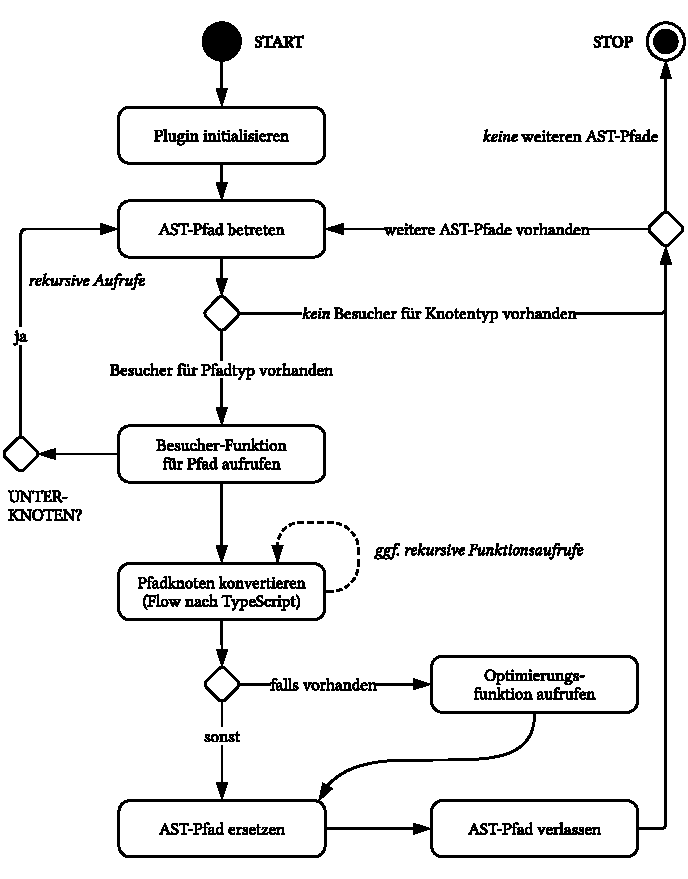
\includegraphics[width=0.85\textwidth]{src/4_Umsetzung/fig/activity-diagram-plugin.pdf}
  \caption{Aktivitätsdiagramm des Transpilers (Babel-Plugin).}
  \label{fig:activity-diagram-plugin}
\end{figure}

% \subsection{Initialisierung des Plugins}

Zu Beginn wird das Plugin wie im Grundlagenteil in Quelltext~\ref{code:babel-plugin-definition} bereits exemplarisch gezeigt initialisiert, d.~h. es wird eine Abbildung der Flow-Knotentypen auf Besucher"=Funktionen definiert. Diese realisieren die Übersetzung von Flow nach TypeScript.
Weiterhin werden die Abhängigkeiten des Plugins spezifiziert. Bei diesen Abhängigkeiten handelt es sich um weitere vorgegebene Babel-Plugins, die benötigt werden, um die Syntax von Flow, JSX~\footnote{Siehe~\citetitle{SOFTWARE:JSX}~\autocite{SOFTWARE:JSX}.} und vorgeschlagenen ECMAScript-Erweiterungen\footnote{Die ECMAScript-Spezifikation wird stetig durch das \textit{Technical Committee 39} (TC39)~\autocite{TC39_COMMITTEE} weiterentwickelt. Vorgeschlagene Erweiterungen der Sprache durchlaufen einen mehrstufigen Standardisierung-Prozess, der schließlich in die Aufnahme in die Spezifikation münden kann~\autocite{TC39_PROCESS}.} einlesen zu können. Auf Grundlage der konkreten Anforderungen bei \textit{TeamShirts} wurden externe Plugins für folgende vorgeschlagene JavaScript-Erweiterungen aktiviert:

\begin{itemize}
  \item Class field declarations for JavaScript~\autocite{ES_PROPOSAL:CLASS_FIELDS}
  \item JavaScript decorators~\autocite{ES_PROPOSAL:DECORATORS}
  \item Dynamic imports~\autocite{ES_PROPOSAL:DYNAMIC_IMPORTS}
\end{itemize}

Daraufhin beginnt die rekursive Traversierung des abstrakten Syntaxbaums der Eingabe"=datei: Jeder Knoten des Baums wird dabei zunächst \textit{betreten} und danach wieder \textit{verlassen}~\autocite{BABEL_HANDBOOK}. Knoten werden verlassen, wenn bei der Beschreitung eines Pfads ein Blatt des Baums erreicht wird und die Traversierung daraufhin auf der höherliegenden Ebene fortgesetzt wird. Im vorliegenden Fall werden die Besucher-Funktionen stets nach Betreten der Pfade aufgerufen.

% die für alle Flow-Knotentypen implementiert wurden
% Da die verschiedenen Knotenarten

\subsection{Transpilierung der Flow-Typen}
  \subsubsection{Transpilierung der Basistypen}
  \subsubsection{Transpilierung der Hilfstypen}
  \subsubsection{Transpilierung der Deklarationen}

\subsection{Weitere Optimierungs-Routinen}
  \subsubsection{Übersetzung gängiger Typimporte}
  \subsubsection{Konvertierung von Klassendekoratoren}
  \label{subsec:class-decorators}

Mapping der Importe (verschiedene Typnamen in Flow und TS), Umwandlung der Decorators usw.

\section{Erweiterung als Kommandozeilenprogramm}

Aufgrund der in Abschnitt~\ref{subsection:requirement:batch-processing} dargelegten Anforderung, dass der Transpiler in der Lage sein muss gesamte Projektverzeichnisse zu verarbeiten (Stapelverarbeitung), ist eine Erweiterung als Kommandozeilenprogramm sinnvoll. Hierdurch können beliebige Dateien und Verzeichnisse eingelesen und deren Übersetzung durch verschiedene Optionen flexibel gesteuert werden. Wie bereits in Abschnitt~\ref{sec:software-architecture} erwähnt benutzt die Konsolenanwendung intern das Babel-Plugin, um die Transpilierung der Flow-Quelltexte nach TypeScript durchzuführen. Aufgaben des Programms sind damit das Einlesen der Eingabe, die Delegation dieser an das Babel-Plugin, die Formatierung des generierten TypeScript-Codes und schließlich die Ausgabe desselben.
Das Werkzeug wurde als ausführbares Node.js-Skript umgesetzt und kann durch das Paketsystem von Node.js installiert werden\footnote{Siehe~\autocite{REFLOW_GITHUB} für detaillierte Installations-Anweisungen.}. Tabelle~\ref{tab:cli-options} listet die verschiedenen Kommandozeile-Optionen des Programms.

\bigskip
\begin{table}[tbh]
  \small
  \begin{tabularx}{\textwidth}{@{}lX@{}}
    \midrule
    \textbf{Option} & \textbf{Beschreibung} \\
    \midrule
    \smallskip
    \texttt{-V -{}-version} & Versionsnummer anzeigen. \\
    \smallskip
    \texttt{-d -{}-dry-run} & Testlauf: Generierten TypeScript-Code auf Standardausgabe schreiben statt in Dateien.\\
    \smallskip
    \texttt{-e -{}-exclude-dirs <pattern ...>} & Kommaseparierte Liste von Verzeichnissen, die von der Transpilierung rekursiv ausgeschlossen werden sollen. \\
    \smallskip
    \texttt{-i -{}-include-pattern <pattern>} & Wildcard-Muster (\textit{glob patterns}) für Eingabedateien. \\
    \smallskip
    \texttt{-r -{}-replace} & Originaldateien (Flow) mit generierten TypeScript-Dateien ersetzen, statt diese beizubehalten. \\
    \smallskip
    \texttt{-D -{}-replace-decorators} & Klassendekoratoren durch verschachtelte Funktionsaufrufe ersetzen (vgl. Abschnitt~\ref{subsec:class-decorators} für Hintergrund). \\
    \smallskip
    \texttt{-h -{}-help} & Hilfe anzeigen. \\
    \midrule
  \end{tabularx}
  \caption{Optionen des Kommandozeilenprogramms}
  \label{tab:cli-options}
\end{table}

% Das Kommandozeilenprogramm wurde in TypeScript geschrieben und kann nach Kompilierung nach JavaScript durch Node.js ausgeführt werden. Es kann wie folgt benutzt werden:



Abbildung~\ref{fig:activity-diagram-cli} auf Seite~\pageref{fig:activity-diagram-cli} zeigt das Aktivitätsdiagramm des Kommandozeilenprogramms.

\begin{figure}[tbp]
  \centering
  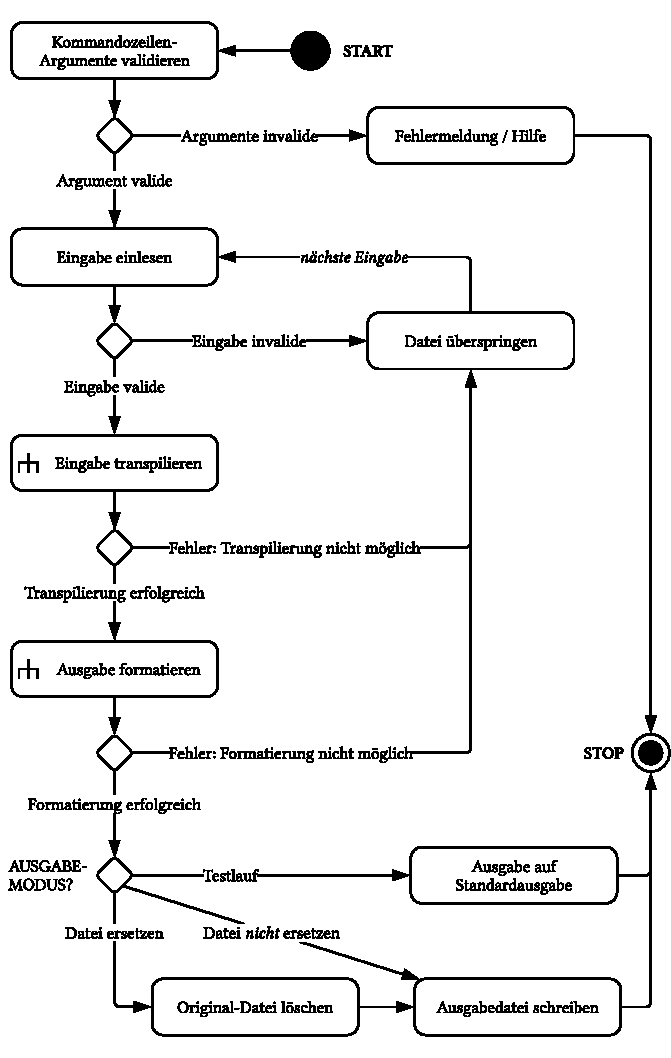
\includegraphics[width=0.85\textwidth]{src/4_Umsetzung/fig/activity-diagram-cli.pdf}
	\caption[Aktivitätsdiagramm des Kommandozeilenprogramms]{Aktivitätsdiagramm des Kommandozeilenprogramms. Vgl. eingebettete Diagramme~\ref{fig:activity-diagram-plugin} \enquote{Eingabe transpilieren} und~\ref{fig:activity-diagram-formatting} \enquote{Ausgabe formatieren}.}
	\label{fig:activity-diagram-cli}
\end{figure}

\section{Formatierung des Ausgabequelltexts}

Eine weitere Problematik, die sich während der Entwicklung des Transpilers gezeigt hat, ist die Formatierung des generierten Ausgabecodes. Da Babel auf Grundlage eines \emph{abstrakten} Syntaxbaums arbeitet, liegt nach der Transformation des Programms keinerlei Information mehr über die ursprüngliche Formatierung des Codes vor\footnote{Ein konkreter Syntaxbaum TODO.}. Die Einrückung und die Position der Leerzeichen und -zeilen gehen somit in der TypeScript-Ausgabe verloren. Es hat sich weiterhin herausgestellt, dass auch die Position der Kommentare nach Anwendung des Babel-Plugins nicht präzise beibehalten wird. Versuche mit der Option \enquote{\texttt{retainLines}}~\autocite{BABEL:GENERATOR} des Codegenerators von Babel erzielten leider nicht das gewünschte Ergebnis. Auch nach Setzen dieser Eigenschaft unterscheidet sich das Format Ausgabequelltext erheblich vom Original. Da die möglichst originalgetreue Formatierung der Ausgabe eine der Anforderungen an den Transpiler ist (vgl. Abschnitt~\ref{subsection:requirement:format}), wurde eine Formatierungs-Routine implementiert, um diese Vorgabe dennoch zu erfüllen. Die Formatierung der Ausgabe wird nach der Transpilierung durch das Kommandozeilenprogramm angestoßen.

\begin{figure}[htbp]
  \centering
  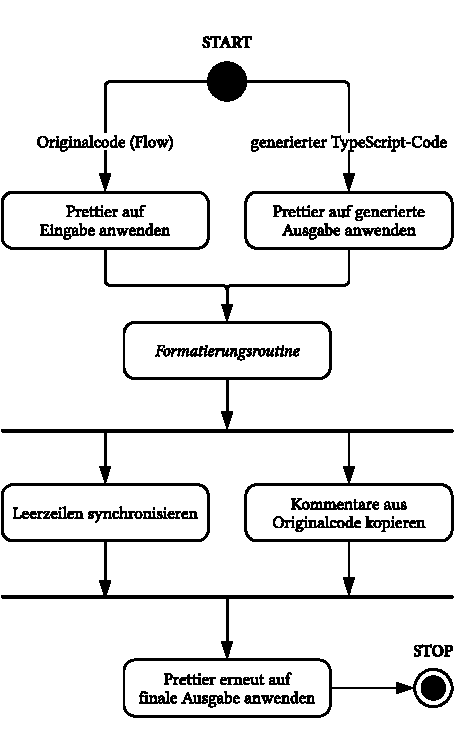
\includegraphics[width=0.55\textwidth]{src/4_Umsetzung/fig/activity-diagram-formatting.pdf}
	\caption[Aktivitätsdiagramm der Formatierung des Ausgabecodes]{Aktivitätsdiagramm der Formatierung des generierten Ausgabecodes.}
	\label{fig:activity-diagram-formatting}
\end{figure}

\medskip
Der konzeptionellen Aufbau der Formatierungs-Funktion wird in Abbildung~\ref{fig:activity-diagram-formatting} dargestellt. Deren Idee ist simpel: Nachdem sowohl die Ein- als auch die Ausgabe in einen vergleichbaren, konsistenten Zustand überführt worden sind, können Leerzeilen und Kommentare einfach übertragen werden.
Zur Herstellung eines solchen Ausgangszustand wird \textit{Prettier} eingesetzt. Prettier ist ein Quelltext-Formatierer, der einen einheitlichen Stil für Sprachen wie JavaScript, Type"=Script, HTML und weitere erzwingt~\autocite{SOFTWARE:PRETTIER}.
Da das weitere Verfahren zeilenbasiert arbeitet, ist es entscheidend, dass die Ausdrücke und Anweisungen der Ein- und Ausgabe gleich Umgebrochen werden. So wird sicher gestellt, dass nur sich entsprechende Zeilen während des Vergleichs betrachtet werden. Versuche haben gezeigt, dass dies bei Anwendung von Prettier nicht in allen Situationen gewährleistet ist. Deshalb wurde das Werkzeug geringfügig modifiziert, um eine größere Konsistenz der Ausgabe von Prettier herzustellen.
Im ersten Schritt der Routine wird diese angepasste Version des Werkzeugs einerseits auf den Originalcode, andererseits auf den generierte TypeScript-Quelltext angewandt. Im Anschluss kann sukzessive über alle Zeilen der Eingabe iteriert und bestehende Leerzeilen an die entsprechende Position in der Ausgabe kopiert werden. Gleichzeitig werden Block- und Zeilenkommentare im ursprünglichen Flow-Programm gesucht und an die gleiche Stelle in den TypeScript-Code eingefügt. Zuletzt wird Prettier erneut auf die Ausgabe angewandt, um verbleibende Probleme wie z.~B. doppelte Leerzeilen zu eliminieren.

% Prettier, synchronisieren der Leerzeilen und Kommentare beschreiben usw.
